\section{BP5-QD problem}
\subsection{Problem description}
\begin{figure}
    \centering
    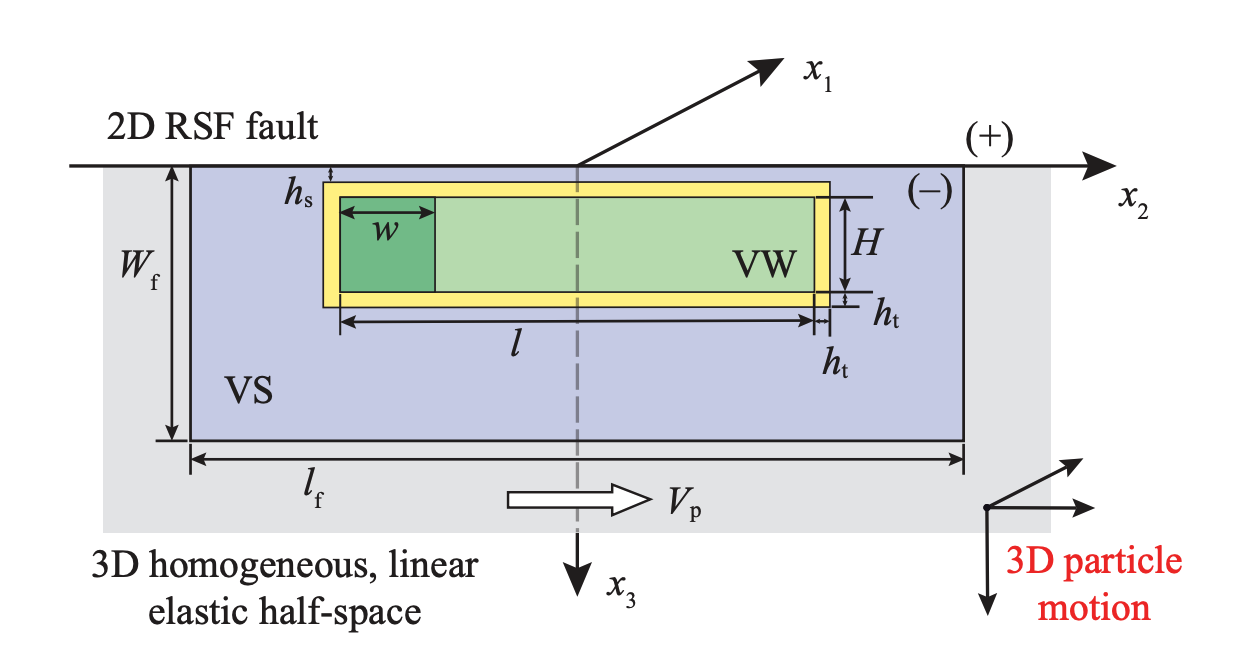
\includegraphics[width=\linewidth]{figures/BP5-figure.png}
    \caption{This benchmark considers 3D motion with a planar fault embedded vertically in a homogeneous, linear elastic whole-space. The fault is governed by rate-and-state friction in the region $0 \leq x_3 \leq W_\text{f}$ and $|x_2| \leq l_f/2$, outside of which it creeps at an imposed constant horizontal rate Vp (gray). The velocity weakening region (the rectangle in light and dark green; $h_s + h_t \leq x_3 \leq h_s + h_t + H$ and $|x_2| \leq l/2)$ is surrounded by a transition zone (yellow) of width ht to velocity strengthening regions (blue). A favorable nucleation zone (dark green square with width $w$) is located at one end of the velocity-weakening patch. \citep{jiang2020seas}}
    \label{fig:BP5-figure}
\end{figure}


\subsection{Boundary and Interface conditions}
At $x_1 = 0$, the fault defines the interfaces.
A free surface lies at $x_3 = 0$, where all components of traction have $0$ value.
This condition is written in the following form
\begin{equation}
    \sigma_{j3}(x_1, x_2, 0, t) = 0,\quad j = 1,2,3
\end{equation}
We assume a ``non-opening condition'' on the fault
\begin{equation}
    u_1(0^+, x_2, x_3, t) = u_1(0^-, x_2, x_3, t)
\end{equation}
For $j=2,3$, we define the slip vector as the jump in horizontal and vertical displacements across the fault.
\begin{equation}
    s_j(x_2, x_3, t) = u_j(0^+, x_2, x_3, t) - u_j(0^-, x_2, x_3, t),\quad j = 2,3
\end{equation}
We require that components of the traction vector be equal and opposite across the fault, which yields three conditions
\begin{align}
    -\sigma_{11} \left(0^+, x_2, x_3, t\right) &= -\sigma_{11} \left(0^-, x_2, x_3, t\right), \\
    \sigma_{21} \left(0^+, x_2, x_3, t\right) &= \sigma_{21} \left(0^-, x_2, x_3, t\right), \\
    \sigma_{31} \left(0^+, x_2, x_3, t\right) &= \sigma_{31} \left(0^-, x_2, x_3, t\right),
\end{align}
We denote these three common values as $\sigma$ (positive means compression), $\tau$ and $\tau_z$ respectively. 
In the simulation, $\tau$ and $\tau_z$ are key values calculated from the displacements and are used in the rate-and-state friction.
We also export the log of these two values to the output files.

Most parameters are given in the problem description. The key value is the rate-and-state friction $a$, given in the following form

\begin{equation}
    a(x_2, x_3) =
\begin{cases} 
a_0, & (h_s + h_t \leq x_3 \leq h_s + h_t + H) \cap (|x_2| \leq l/2) \\
a_{\text{max}}, & (0 \leq x_3 \leq h_s) \cup (h_s + 2h_t + H \leq x_3 \leq W_f) \\ & \cup (l/2 + h_t \leq |x_2| \leq l_f/2) \\
a_0 + r(a_{\text{max}} - a_0), & \text{other regions}
\end{cases}
\end{equation}
where $r = \max(|x_3 - h_s - h_t - H/2| - H/2, |x_2| - l/2)/h_t$.


Outside the domain $\Sigma_f$ ($|x_3| > W_\text{f}$ or $|x_2| > l_\text{f} / 2$ as denoted in the grey region in the \autoref{fig:BP5-figure}), the fault creeps horizontally at an imposed constant rate
\begin{align}
    V_2(x_2, x_3, t) &= V_\text{p} \\
    V_3(x_2, x_3, t) &= 0
\end{align}
where $V_\text{p}$ is the plate rate.

We also need to specify the initial conditions for the simulation.
We assume that slip on the fault separating identical materials does not change normal traction, so $\sigma_n$ remains constant.

The initial state and prestress on the fault is chosen so that the model can start with a uniform fault slip rate, given by $\textbf{V} = [V_\text{init}, V_\text{zero}]$ where $V_\text{zero}$ is chosen as $10^{-20}m/s$ to avoid infinite log values in the output, and $\boldsymbol{\tau}^0 = \tau^0 \textbf{V} / V$.

The initial state variable is chosen as the steady state at slip rate $V_\text{init}$ over the entire fault 
\begin{equation}
    \theta(x_2, x_3, 0) = L / V_\text{init}
\end{equation}

For the BP5-QD problem, we also need to specify an initial value for the slip, which we set to be zero.
\begin{equation}
    s_j(x_2, x_3, t) = 0, j = 2, 3
\end{equation}
The scalar pre-stress $\tau^0$ is chosen as the steady-state stress
\begin{equation}
    \tau^0 = \bar{\sigma}_\text{n} a \sinh^{-1}[\frac{V_\text{init}}{2V_0}\exp(\frac{f_0 + b\ln(V_0/V_\text{init}}{a})] + \eta V_\text{init}
\end{equation}
To break the symmetry of the problem and facilitate comparisons of different simulations, we choose a small region as a favorable location for nucleation to impose a smaller critical slip distance ($L=0.13m$) and higher initial slip rate along the $x_2$-direction ($V_i = 0.03 m/s$) while keeping the initial state variable $\theta(x_2, x_3, 0)$ unchanged. The means we impose higher pre-stress along the $x_2$-direction.

We use the recommended parameters from the problem description and perform initial simulations for 1800 years.

\subsection{SBP-SAT formulations for BP5-QD}
For this 3D problem, we use SBP-SAT methods similar to \citep{ALMQUIST2021109842} to formulate our linear system.
To solve the linear elasticity in 3D, we need to solve for the displacements in $x$, $y$, and $z$ directions for each point.
We denote the displacement vector as $\boldsymbol{u} = [u_1, u_2, u_3]$.
To turn the tensor formulation from \citep{ALMQUIST2021109842} into a matrix formulation for iterative solvers,  we first stack the displacements for a point in $x$, $y$, $z$ directions, and then for all points in $x$, $y$, and $z$ directions.
We label the faces for 3D simulation in the following order as shown in \autoref{fig:3d_problem}

\begin{figure}
    \centering
    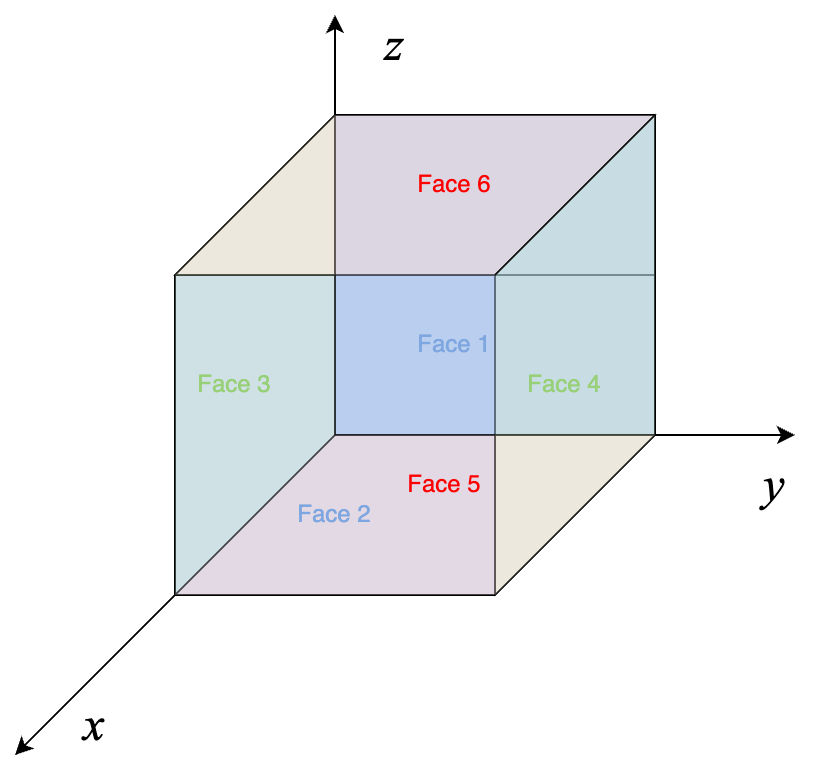
\includegraphics[width=\linewidth]{figures/3D_problem.png}
    \caption{We set up the 3D coordinate and denote faces 1 to 6 using different colors. Face 1 and Face 2 are perpendicular to the x-axis denoted using blue color. Face 3 and Face 4 are perpendicular to the y-axis denoted using green color. Face 5 and Face 6 are perpendicular to the z-axis denoted using red color. We impose Dirichlet boundary conditions on Face 1 and Face 2. For Face 3 to Face 6, we impose traction-free (Neumann) condition.} 
    \label{fig:3d_problem}
\end{figure}

The first step is to derive values for $\sigma$ tensor in 3D.

\begin{align}
    \sigma_{11} = K\epsilon_{kk} + 2\mu (\epsilon_{11} - \frac{1}{3}\epsilon_{kk}) &= (K - \frac{2}{3}\mu)( \frac{\partial u_1}{\partial x_1} + \frac{\partial u_2}{\partial x_2} + \frac{\partial u_3}{\partial x_3}) + 2\mu \frac{\partial u_1}{\partial x_1} \\
    \sigma_{12} = 2\mu \epsilon_{12} &= \mu(\frac{\partial u_1}{\partial x_2} + \frac{\partial u_2}{\partial x_1}) \\
    \sigma_{13} = 2\mu \epsilon_{13} &= \mu(\frac{\partial u_1}{\partial x_3} + \frac{\partial u_3}{\partial x_1}) \\
    \sigma_{21} = 2\mu \epsilon_{21} &= \mu(\frac{\partial u_2}{\partial x_1} + \frac{\partial u_1}{\partial x_2}) \\
    \sigma_{22} = K\epsilon_{kk} + 2\mu (\epsilon_{22} - \frac{1}{3}\epsilon_{kk}) &= (K - \frac{2}{3}\mu)( \frac{\partial u_1}{\partial x_1} + \frac{\partial u_2}{\partial x_2} + \frac{\partial u_3}{\partial x_3}) + 2\mu \frac{\partial u_2}{\partial x_2} \\
    \sigma_{23} = 2\mu \epsilon_{13} &= \mu(\frac{\partial u_2}{\partial x_3} + \frac{\partial u_3}{\partial x_2}) \\
    \sigma_{31} = 2\mu \epsilon_{31} &= \mu(\frac{\partial u_3}{\partial x_1} + \frac{\partial u_1}{\partial x_3}) \\
    \sigma_{32} = 2\mu \epsilon_{32} &= \mu(\frac{\partial u_3}{\partial x_2} + \frac{\partial u_2}{\partial x_3}) \\
    \sigma_{33} = K\epsilon_{kk} + 2\mu (\epsilon_{33} - \frac{1}{3}\epsilon_{kk}) &= (K - \frac{2}{3}\mu)( \frac{\partial u_1}{\partial x_1} + \frac{\partial u_2}{\partial x_2} + \frac{\partial u_3}{\partial x_3}) + 2\mu \frac{\partial u_3}{\partial x_3}
    \label{eqn:sigma-tensor}
\end{align}


Here, we also use $1,2,3$ to denote the components of $\sigma$ in $x,y,z$ directions to simplify the notation.
Then we can rewrite governing equations in terms of the $x,y,z$ components.

\begin{align}
    \rho \frac{\partial^2{u_1}}{\partial{t^2}} &= \frac{\partial \sigma_{11}}{\partial x_1} + \frac{\partial \sigma_{12}}{\partial x_{2}} + \frac{\partial \sigma_{13}}{\partial x_{3}} \nonumber \\
    &= (K - \frac{2}{3}\mu)( \frac{\partial^2 u_1}{\partial x_1^2} + \frac{\partial^2 u_2}{\partial x_1 \partial x_2} + \frac{\partial^2 u_3}{\partial x_1 \partial x_3}) + 2\mu \frac{\partial^2u_1}{\partial x_1^2} \nonumber \\
        & + \mu(\frac{\partial^2 u_1}{\partial x_2^2} + \frac{\partial^2u_2}{\partial x_2 \partial x_1})
        + \mu(\frac{\partial^2 u_1}{\partial x_3^2} + \frac{\partial^2u_3}{\partial x_3 \partial x_1}) \\
    \rho \frac{\partial^2{u_2}}{\partial{t^2}} &= \frac{\partial \sigma_{21}}{\partial x_1} + \frac{\partial \sigma_{22}}{\partial x_{2}} + \frac{\partial \sigma_{23}}{\partial x_{3}} \nonumber \\
    &= \mu(\frac{\partial^2u_2}{\partial x_1^2} + \frac{\partial^2 u_1}{\partial x_1 \partial x_2})
    + (K - \frac{2}{3}\mu)( \frac{\partial^2 u_1}{\partial x_2 \partial x_1} + \frac{\partial^2 u_2}{\partial x_2^2} + \frac{\partial^2 u_3}{\partial x_2 \partial x_3}) \nonumber \\
    &+ 2\mu \frac{\partial^2u_2}{\partial x_2^2} 
    + \mu(\frac{\partial^2u_2}{\partial x_3^2} + \frac{\partial^2 u_3}{\partial x_3 \partial x_2}) \\
    \rho \frac{\partial^2{u_3}}{\partial{t^2}} & = \frac{\partial \sigma_{31}}{\partial x_1} + \frac{\partial \sigma_{32}}{\partial x_{2}} + \frac{\partial \sigma_{33}}{\partial x_{3}} \nonumber \\
    &= \mu(\frac{\partial^2u_3}{\partial x_1^2} + \frac{\partial^2 u_1}{\partial x_1 \partial x_3}) \nonumber
    + \mu(\frac{\partial^2 u_3}{\partial x_2^2} + \frac{\partial^2u_2}{\partial x_2 \partial x_3}) \\
    & + (K - \frac{2}{3}\mu)( \frac{\partial^2 u_1}{\partial x_3 \partial x_1}   + \frac{\partial^2 u_2}{\partial x_3 \partial x_2} + \frac{\partial^2 u_3}{\partial x_3^2}) + 2\mu \frac{\partial^2u_3}{\partial x_3^2} 
    \label{eqn:components}
\end{align}

We can use them to impose the SAT terms for displacements in $x, y, z$ directions using formulations from \citep{ALMQUIST2021109842}.
For Neuman boundary conditions, we have
\begin{align}
    SAT_1 = &-H^{-1} [e_3 H_3 (e_3^T [T_{11}^3 u_1 + T_{12}^3 u_2 + T_{13}^3 u_3] - g_1^3)] \nonumber \\
&- H^{-1} [e_4 H_4 (e_4^T [T_{11}^4 u_1 + T_{12}^4 u_2 + T_{13}^4 u_3] - g_1^4)] \nonumber \\
&- H^{-1} [e_5 H_5 (e_5^T [T_{11}^5 u_1 + T_{12}^5 u_2 + T_{13}^5 u_3] - g_1^5)] \nonumber \\
&- H^{-1} [e_6 H_6 (e_6^T [T_{11}^6 u_1 + T_{12}^6 u_2 + T_{13}^6 u_3] - g_1^6)] \\
SAT_2 = &-H^{-1} [e_3 H_3 (e_3^T [T_{21}^3 u_1 + T_{22}^3 u_2 + T_{23}^3 u_3] - g_2^3)] \nonumber \\
& - H^{-1} [e_4 H_4 (e_4^T [T_{21}^4 u_1 + T_{22}^4 u_2 + T_{23}^4 u_3] - g_2^4)] \nonumber \\
& - H^{-1} [e_5 H_5 (e_5^T [T_{21}^5 u_1 + T_{22}^5 u_2 + T_{23}^5 u_3] - g_2^5)] \nonumber \\
& - H^{-1} [e_6 H_6 (e_6^T [T_{21}^6 u_1 + T_{22}^6 u_2 + T_{23}^6 u_3] - g_2^6)] \\
SAT_3 = &-H^{-1} [e_3 H_3 (e_3^T [T_{31}^3 u_1 + T_{32}^3 u_2 + T_{33}^3 u_3] - g_3^3)] \nonumber\\
& - H^{-1} [e_4 H_4 (e_4^T [T_{31}^4 u_1 + T_{32}^4 u_2 + T_{33}^4 u_3] - g_3^4)] \nonumber\\
& - H^{-1} [e^5 H_5 (e_5^T [T_{31}^5 u_1 + T_{32}^5 u_2 + T_{33}^5 u_3] - g_3^5)] \nonumber\\
& - H^{-1} [e^6 H_6 (e_6^T [T_{32}^6 u_1 + T_{32}^6 u_2 + T_{33}^6 u_3] - g_3^6)]
\label{eqn:neumann-condition}
\end{align}

For Dirichlet conditions, we have
\begin{align}
    \tilde{SAT_1} &= H^{-1} (T_{11}^1 - Z_{11}^1)^T e_1 H_1 (e_1^T u_1 - g_1^1) \nonumber \\
    &+ H^{-1} (T_{21}^1 - Z_{21}^1)^T e_1 H_1 (e_1^T u_2 - g_2^1) \nonumber\\ 
    &+ H^{-1} (T_{31}^1 - Z_{31}^1)^T e_1 H_1 (e_1^T u_3 - g_3^1) \nonumber\\
    &+ H^{-1} (T_{11}^2 - Z_{11}^2)^T e_2 H_2 (e_2^T u_1 - g_1^2) \nonumber\\
    &+ H^{-1} (T_{21}^2 - Z_{21}^2)^T e_2 H_2 (e_2^T u_2 - g_2^2) \nonumber\\
    &+ H^{-1} (T_{31}^2 - Z_{31}^2)^T e_2 H_2 (e_2^T u_3 - g_3^2) \\
    \tilde{SAT_2} &= H^{-1} (T_{12}^1 - Z_{12}^1)^T e_1 H_1 (e_1^T u_1 - g_1^1) \nonumber \\
    & + H^{-1} (T_{22}^1 - Z_{22}^1)^T e_1 H_1 (e_1^T u_2 - g_2^1) \nonumber \\
    & + H^{-1} (T_{32}^1 - Z_{32}^1)^T e_1 H_1 (e_1^T u_3 - g_3^1) \nonumber \\
    & + H^{-1} (T_{12}^2 - Z_{12}^2)^T e_2 H_2 (e_2^T u_1 - g_1^2) \nonumber \\
    & + H^{-1} (T_{22}^2 - Z_{22}^2)^T e_2 H_2 (e_2^T u_2 - g_2^2) \nonumber \\ 
    & + H^{-1} (T_{32}^2 - Z_{32}^2)^T e_2 H_2 (e_2^T u_3 - g_3^2) \\
    \tilde{SAT_3} &= H^{-1} (T_{13}^1 - Z_{13}^1)^T e_1 H_1 (e_1^T u_1 - g_1^1) \nonumber \\
    & + H^{-1} (T_{23}^1 - Z_{23}^1)^T e_1 H_1 (e_1^T u_2 - g_2^1) \nonumber \\ 
    & + H^{-1} (T_{33}^1 - Z_{33}^1)^T e_1 H_1 (e_1^T u_3 - g_3^1) \nonumber \\
    & + H^{-1} (T_{13}^2 - Z_{13}^2)^T e_2 H_2 (e_2^T u_1 - g_1^2) \nonumber \\
    & + H^{-1} (T_{23}^2 - Z_{23}^2)^T e_2 H_2 (e_2^T u_2 - g_2^2) \nonumber \\
    & + H^{-1} (T_{33}^2 - Z_{33}^2)^T e_2 H_2 (e_3^T u_3 - g_3^2)
    \label{eqn:dirichlet-condition}
\end{align}

Detailed formulation of these matrices will be provided in the code for paper submission in the future.
% \subsection{Discretization and parameters selection}


\subsection{Results}
We discretize the problem on a truncated 128km $\times$ 128km $\times$ 128 km domain. The simulation parameters are chosen to be the values in \citep{jiang2020seas}. 
We export results on stations on the fault according to the problem description. We run our simulations for 1800 years and compare our results with results from other researchers on similar problems.

We compare our results with results obtained using boundary element methods (BEMs) from Cattania's group. BEMs only require solving problems on the fault surface, and does not require domain truncation. Previous results have shown that domain truncation in volume-based methods would affect earthquake cycles
We first look at the changes in shear stress along the slip direction for a sample location on the fault. We compare our results with Cattania's group using boundary element methods and plot the result in \autoref{fig:bp5-shearstress}. We see similar ranges of state variables and similar behaviors of jumps in state variables during the transition between aseismic slips and seismic slips. We then compare the slip for the same location on the fault and plot them in \autoref{fig:bp5-slip2}.

\begin{figure}
    \centering
    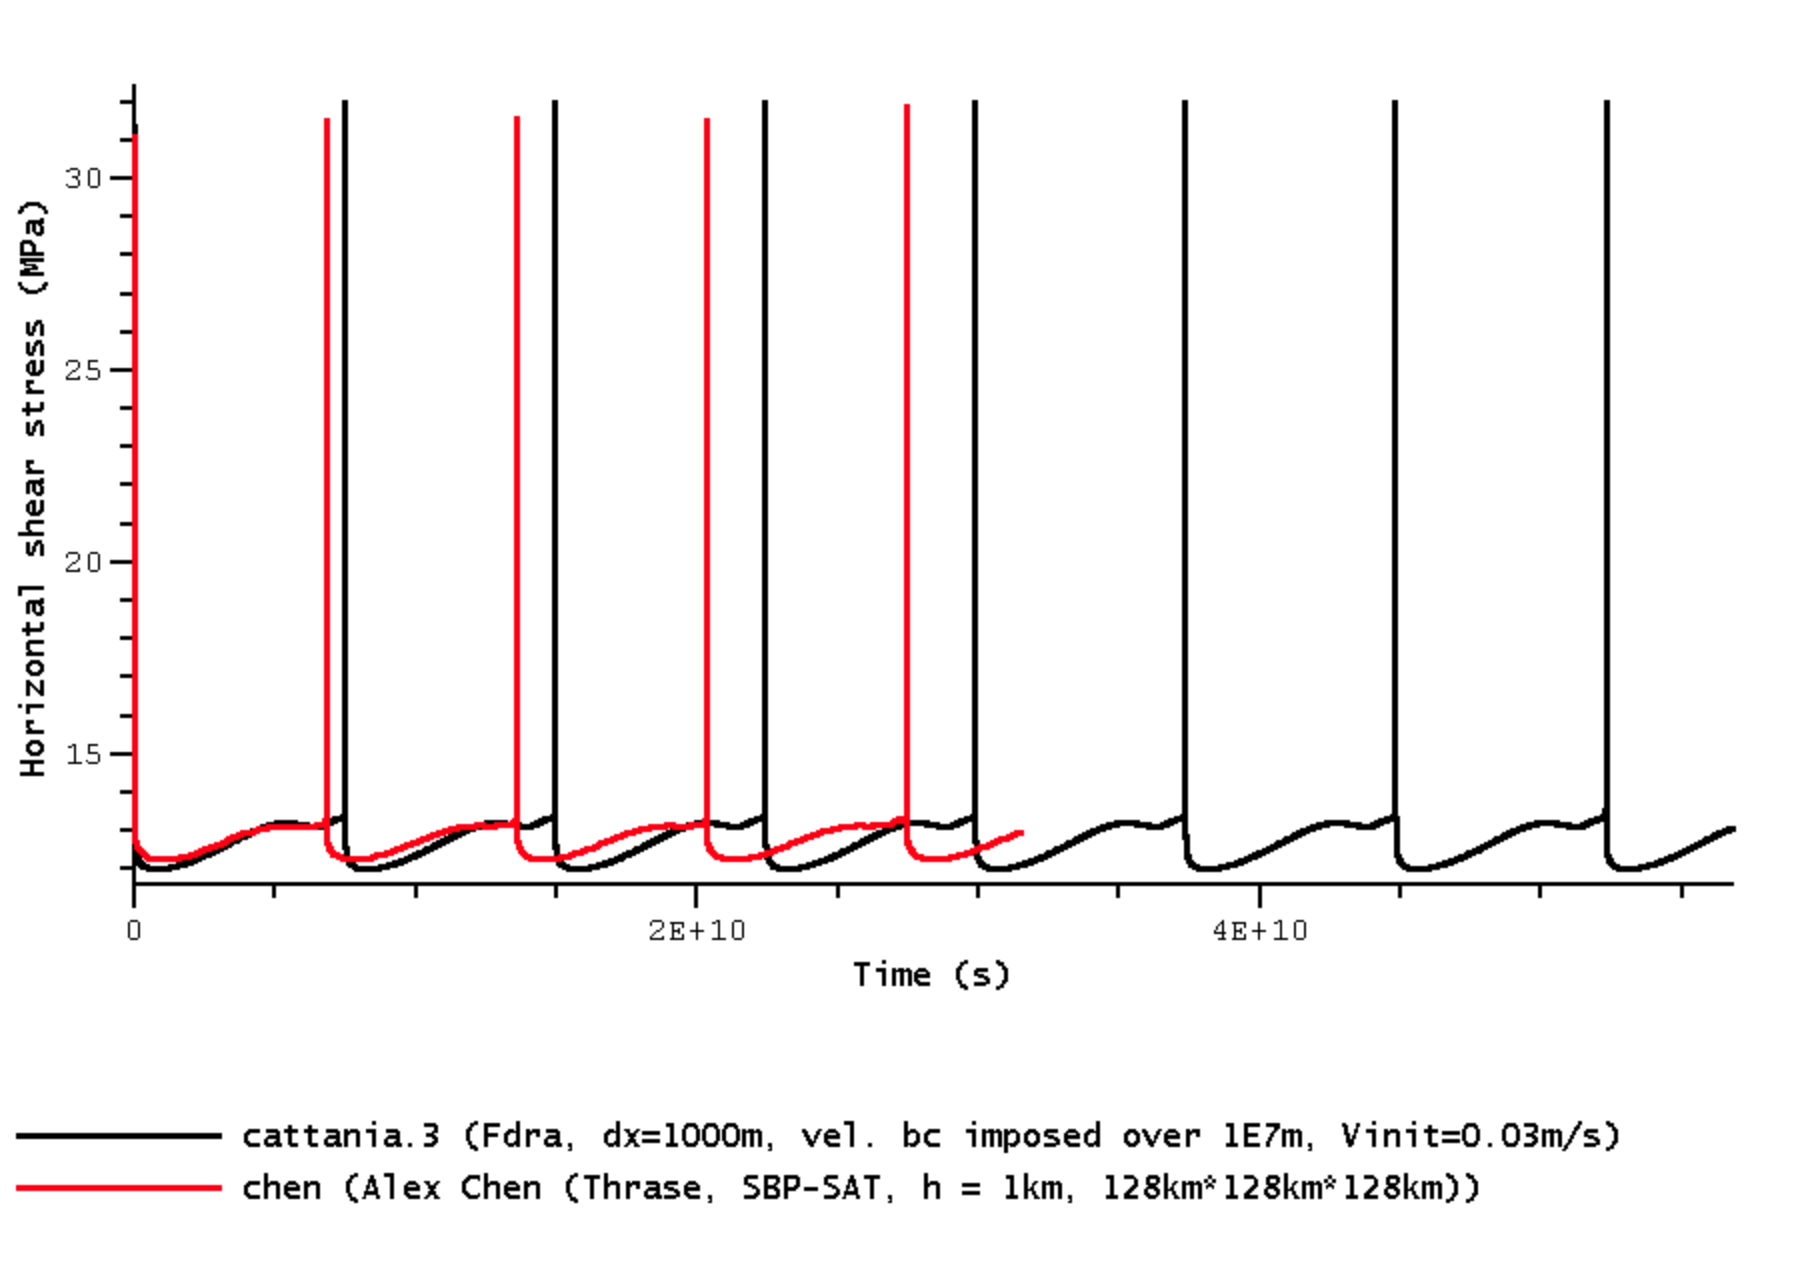
\includegraphics[width=\linewidth]{figures/sample-shearstress.png}
    \caption{Comparison of shear stress along slip directions}
    \label{fig:bp5-shearstress}
\end{figure}

\begin{figure}
    \centering
    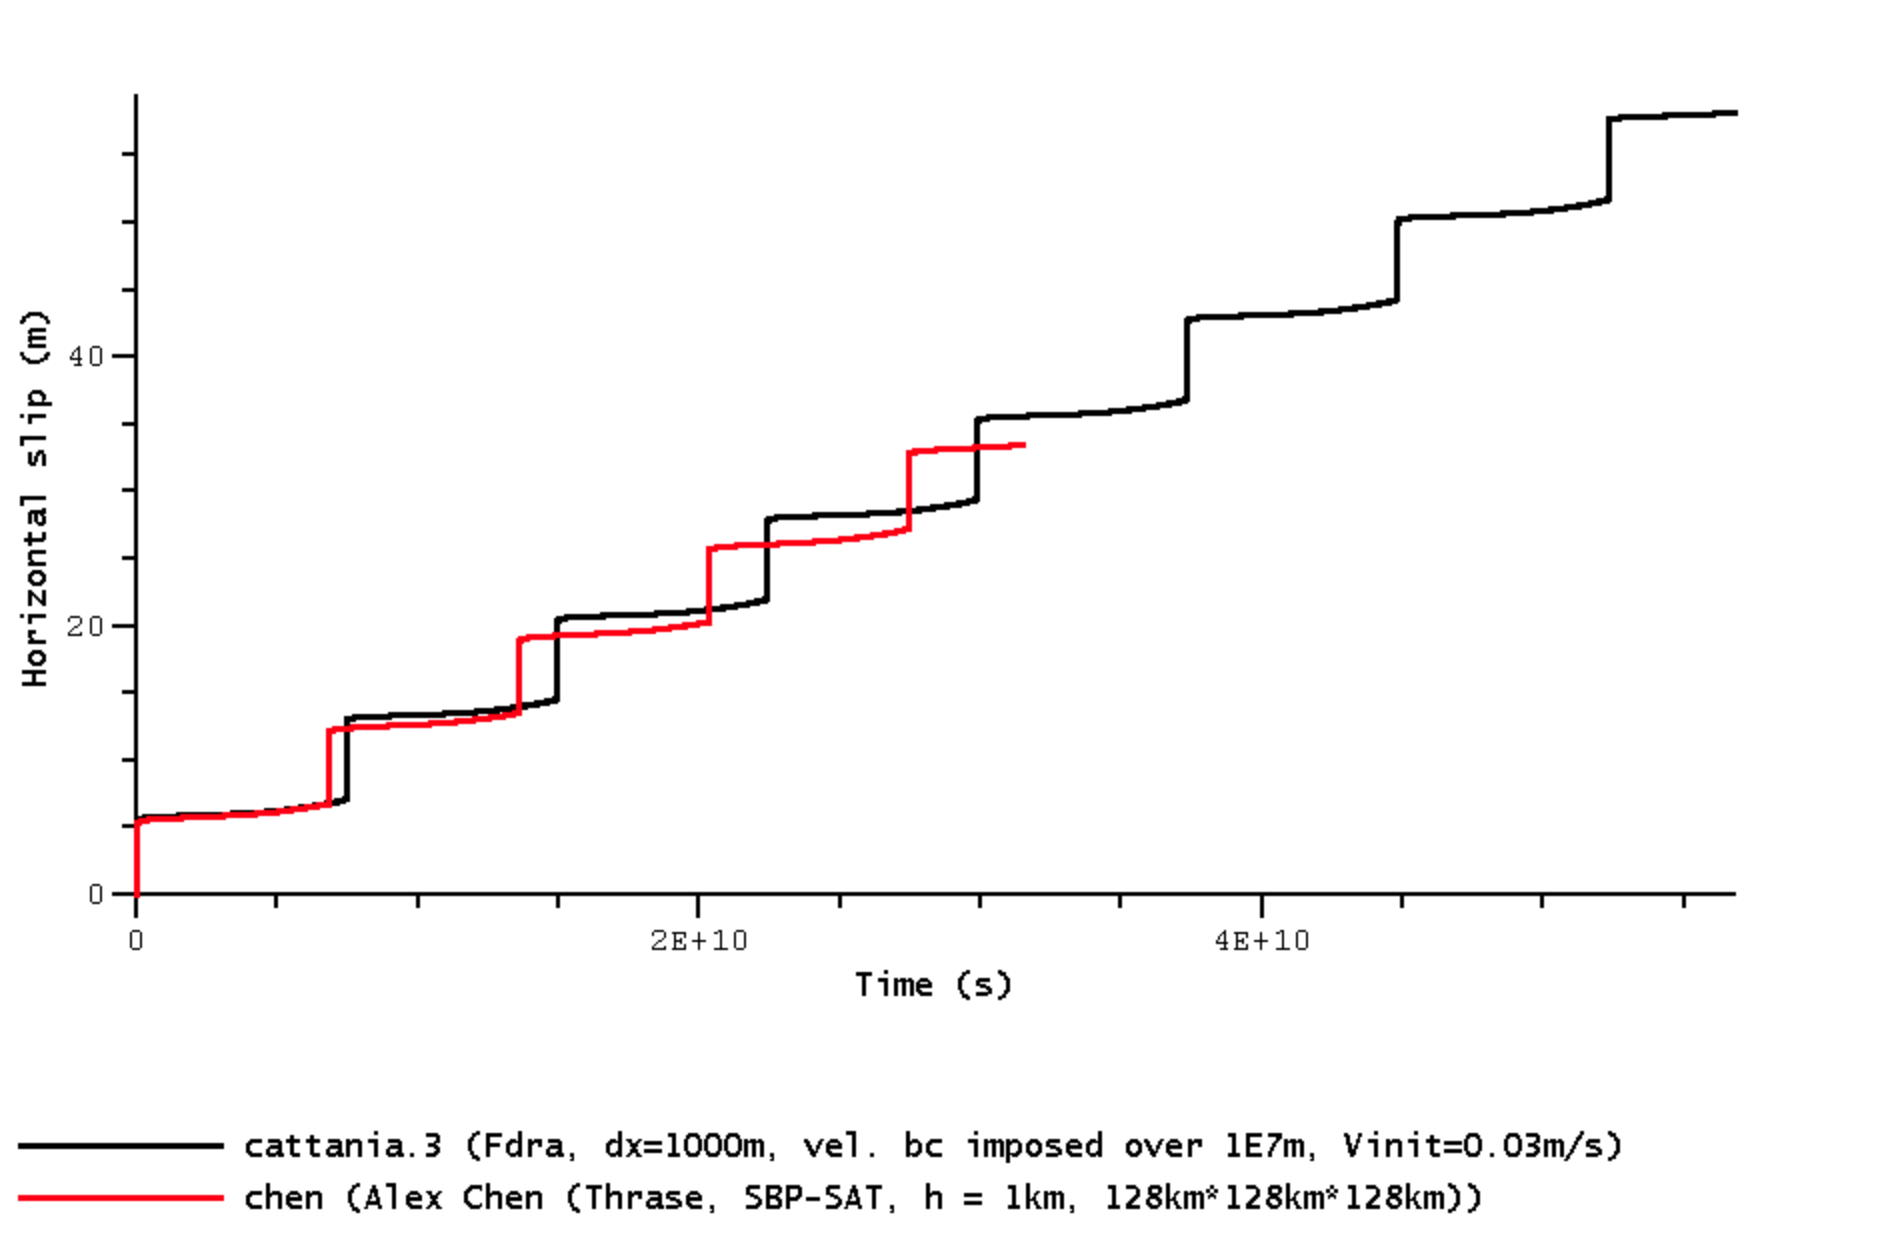
\includegraphics[width=\linewidth]{figures/sample-slip-2.png}
    \caption{Comparison of shear stress along slip directions}
    \label{fig:bp5-slip2}
\end{figure}

Last we look at changes in the state variable for two sample locations on the fault, one inside and one outside of the nucleation favorable region. The figures are shown in \autoref{fig:state-inside} and \autoref{fig:state-outside}. 
\begin{figure}
    \centering
    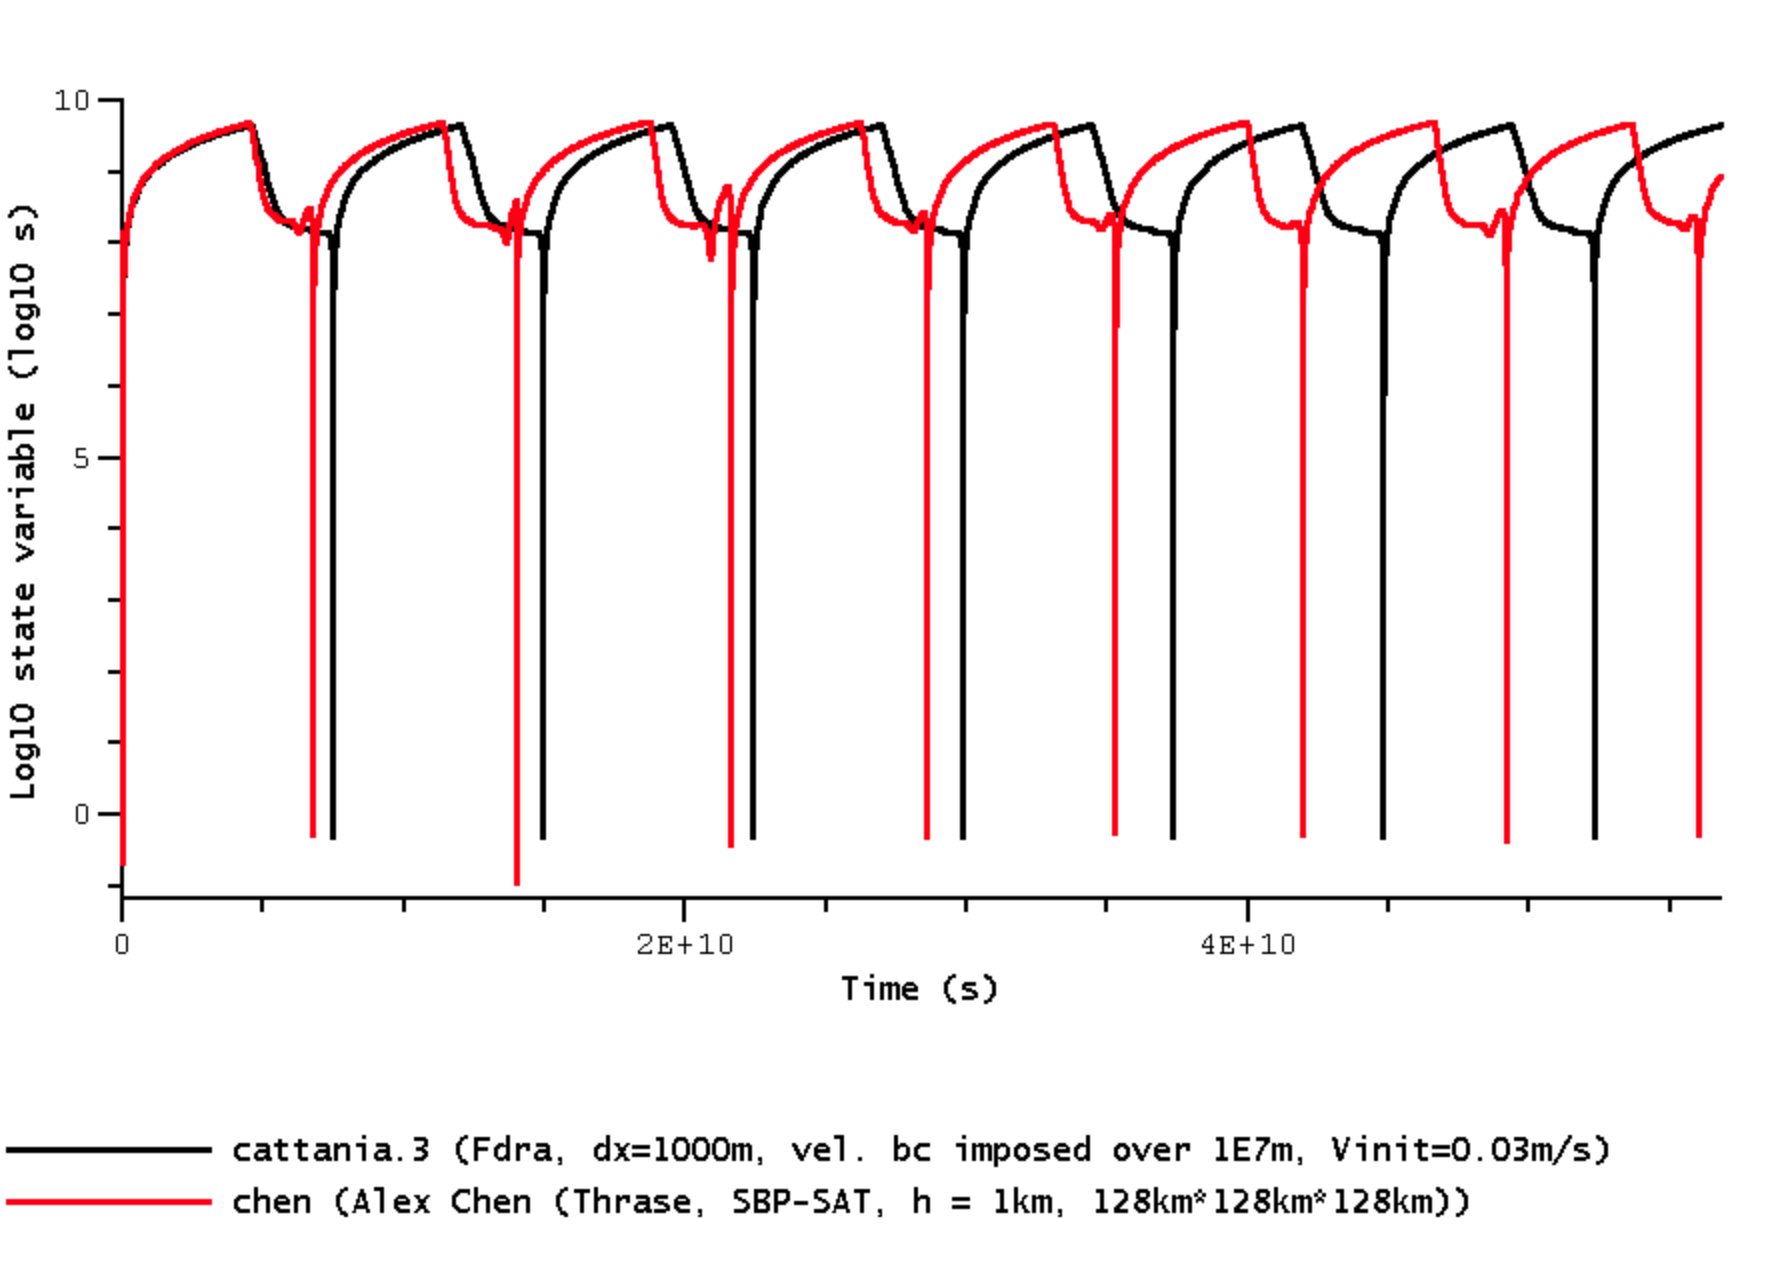
\includegraphics[width=\linewidth]{figures/state-variable-nucleation.png}
    \caption{Comparison of the state variable inside the nucleation favorable region}
    \label{fig:state-inside}
\end{figure}

\begin{figure}
    \centering
    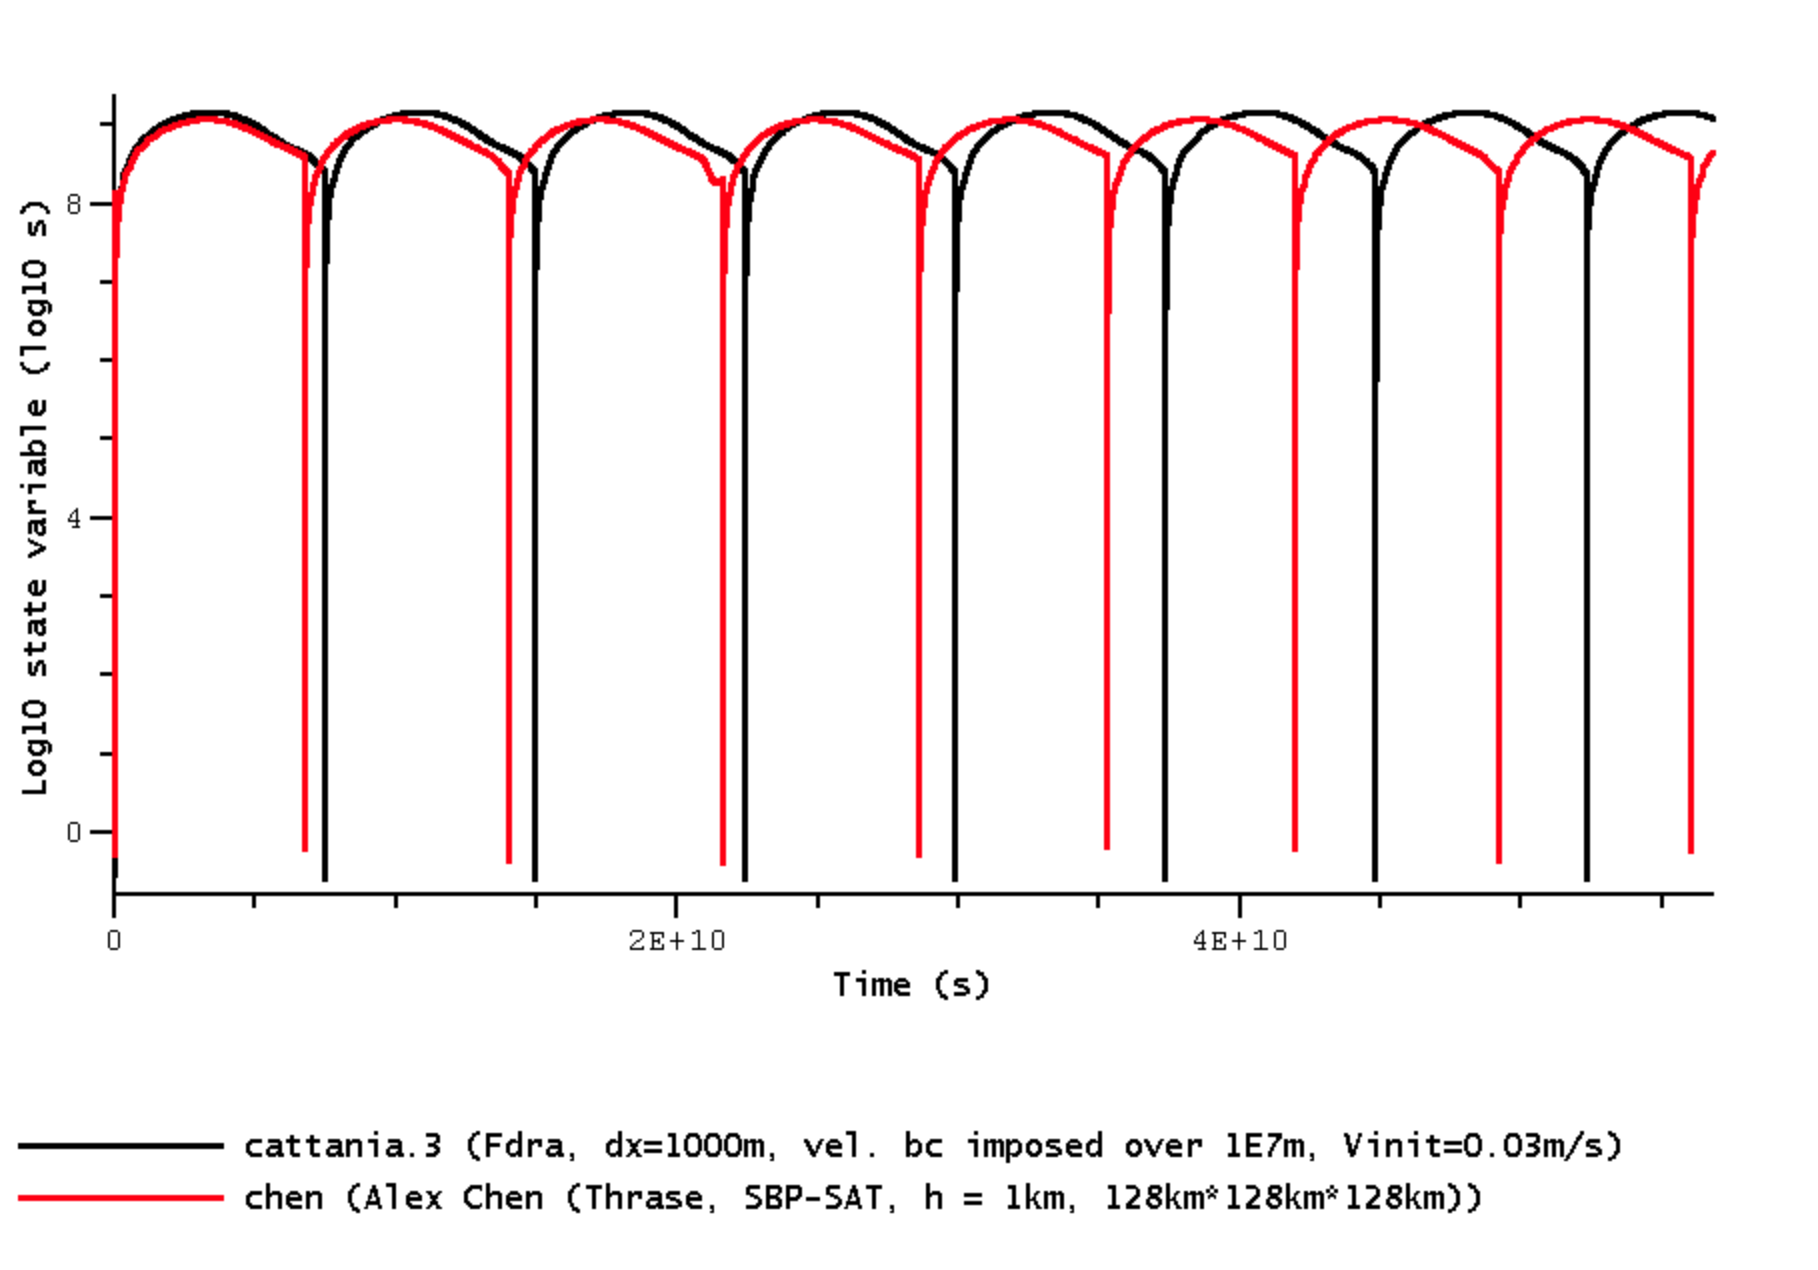
\includegraphics[width=\linewidth]{figures/state-variable-outside-nucleation.png}
    \caption{Comparison of the state variable outside the nucleation favorable region}
    \label{fig:state-outside}
\end{figure}



Preliminary results have shown agreement in the modeling of the same problems using different methods.
Both our model and the model from comparison group can capture different behaviors of earthquakes for fault stations inside and outside of the nucleation favorable regions.
Current results from other simulations are mainly based on boundary element methods, which take hours to run.
Our methods are volume-based and have more than 100 times higher degrees of freedom.
With the GPU-accelerated MGCG as a solver, our simulation time is cut to around ~8 hours, with around $0.2s$ for each round of solving linear system and updating values. 
This is down from years of estimated time using direct methods if we have sufficient large enough memory for matrix factorization.